%%%%%%%%%%%%%%%%%%%%%%%%%%%%%%%%%%%%%%%%%%%%%%%%%%%%%%
\VideoClassification[column=2, colour=red]
%%%%%%%%%%%%%%%%%%%%%%%%%%%%%%%%%%%%%%%%%%%%%%%%%%%%%%

\midTitle{Schema Types}
\begin{frame}
\frametitle{Schema Types}
	\begin{itemize}[<+->]
		\item Star Schema.
		\item Snowflake Schema.
	\end{itemize}

\end{frame}
%%%%%%%%%%%%%%%%%%%%%%%%%%%%%%%%%%%%%%%%%%%%%%%%%%%%%%
%%%%%%%%%%%%%%%%%%%%%%%%%%%%%%%%%%%%%%%%%%%%%%%%%%%%%%
\midTitle{Schema Types: Star Schema}
\begin{frame}
	\frametitle{Star Schema Characteristics}
	\begin{itemize}[<+->]
		\item \textbf{Simplicity}: It is the simplest type of DWH schemas.
		\item \textbf{Query effectiveness}: Because of simplicity, It needs less join to query the data (It is optimized to query large dataset).
		\item \textbf{Data Redundancy and Large Table Size}: Due to de-normalization, it has a data redundancy, and the table size is huge.
		\item \textbf{Most} used and \textbf{widely} supported.
	\end{itemize}
\end{frame}
%%%%%%%%%%%%%%%%%%%%%%%%%%%%%%%%%%%%%%%%%%%%%%%%%%%%%%
\begin{frame}
\frametitle{Star Schema Characteristics}
	\begin{itemize}[<+->]
		\item Dimensions represented by one one-dimension table.
		\item The dimension table are not joined to each other
		\item The fact table would contain key and measure.
		\item Data integrity is not enforced due to the de-normalized structure.
	\end{itemize}
\end{frame}
%%%%%%%%%%%%%%%%%%%%%%%%%%%%%%%%%%%%%%%%%%%%%%%%%%%%%%
\begin{frame}
\frametitle{Schema Types: Star Schema Example}
\begin{tikzpicture}[every node/.style={font=\ttfamily}, node distance=1.4in,scale=.75, every node/.style={scale=0.75}]
%https://tex.stackexchange.com/questions/133754/creating-crows-foot-style-e-r-diagrams-rather-than-chen-style-ones
\matrix  [entity=Usage, entity anchor=Usage-id]  {
	\properties{
		id,
		cust-id (FK),
		cal-id (FK), 
		loc-id (FK),
		promo-id (FK),
		date-id (FK),
		TotalInCalls (agg),
		TotalOutCalls (agg),
		TotalAmount (agg)
	}
};


\matrix  [entity=CellLookup, above left=of Usage-id, entity anchor=CellLookup-id]  {
	\properties{
		id,
		celltype,
		vendorname,
		street,
		city,
		state,
		zip
	}
};
\matrix  [entity=Promotion, below left=of Usage-id,yshift=10ex, entity anchor=Promotion-id]  {
	\properties{
		id,
		promotype,
		promodesc,
		value,
		startdate,
		enddate
	}
};

\matrix [entity=CustomerProfile, below right=of Usage-id,yshift=10ex, entity anchor=CustomerProfile-id]  {
	\properties{
		id, 
		gender, 
		age, 
		nationality,
		firstname,
		lastname
	}
};


\matrix  [entity=Calendar, above right=of Usage-id, entity anchor=Calendar-id]  {
	\properties{
		id,
		date,
		day,
		week,
		month,
		qtr,
		year
	}
};

\draw [one to one] (Usage-id)  to (CustomerProfile-id);
\draw [one to one] (Usage-id)  to (Calendar-id);
\draw [one to one] (Usage-id)  to (CellLookup-id);
\draw [one to one] (Usage-id)  to (Promotion-id);

\end{tikzpicture}
%%%%%%%%%%%%%%%%%%%%%%%%%%%%%%%%%%%%%%%%%%%%%%%%%%%%%%%%%%%%%%%%%%%%%%%%%%%
%%% Local Variables:
%%% mode: latex
%%% TeX-master: "../../main.tex"
% !TeX root = ../../main.tex
%%% TeX-engine: xetex
%%% End:

\end{frame}
%%%%%%%%%%%%%%%%%%%%%%%%%%%%%%%%%%%%%%%%%%%%%%%%%%%%%%%
\midTitle{Schema Types: Snowflake Schema}
\begin{frame}
	\frametitle{What is Snowflake?}
	\begin{figure}
	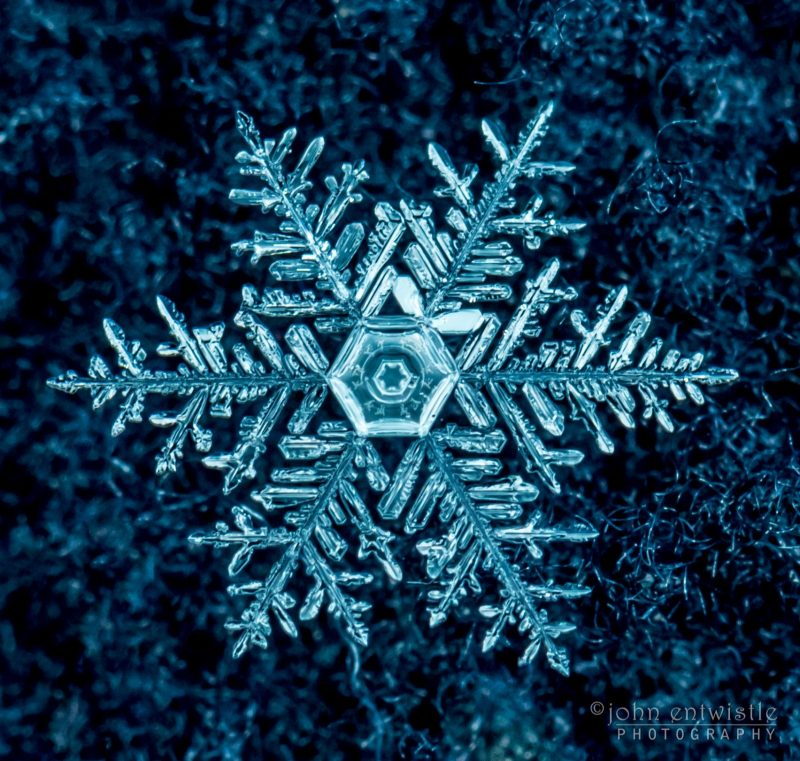
\includegraphics[scale=0.25]{Ch01-Introduction-data-management/12-Data-Model/04-Data-Model-Schema-Types/Figures/snowflake-real.jpg}
	\caption{Snowflake Photo taken from  \href{https://earthsky.org/earth/best-snowflakes-photos-from-earthsky-friends}{https://earthsky.org}}
	\end{figure}
\end{frame}
%%%%%%%%%%%%%%%%%%%%%%%%%%%%%%%%%%%%%%%%%%%%%%%%%%%%%%%
\begin{frame}
	\frametitle{What is Snowflake?}
	\begin{figure}
		
\includegraphics[scale=0.5]{Ch01-Introduction-data-management/12-Data-Model/04-Data-Model-Schema-Types/Figures/Snowflakes-PNG-File.png}
		\caption{Snowflake Simple Design}
	\end{figure}
\end{frame}
%%%%%%%%%%%%%%%%%%%%%%%%%%%%%%%%%%%%%%%%%%%%%%%%%%%%%%%
\begin{frame}
	\frametitle{What is Snowflake?}
	\begin{figure}
		
\includegraphics[scale=0.2]{Ch01-Introduction-data-management/12-Data-Model/04-Data-Model-Schema-Types/Figures/Frozen-Snowflake-PNG-File.png}
		\caption{Snowflake Final Design}
	\end{figure}
\end{frame}
%%%%%%%%%%%%%%%%%%%%%%%%%%%%%%%%%%%%%%%%%%%%%%%%%%%%%%%
\begin{frame}
\frametitle{Star Schema Characteristics}
	\begin{itemize}
		\item \textbf{Extension}: Snowflake is an extension of the Star Schema.
		\item \textbf{Normalized}: Dimension tables are normalized; this means every dimension may expand into additional tables.
		\item \textbf{Disk Space Efficiency}:  Due to its normalization methodology, it uses less desk space, which enhances the query as we scan less data size.
		\item \textbf{Complicated}: Due to the normalization query needs to join more table in some cases to get the data which reduces the performance.
	\end{itemize}

\end{frame}

%%%%%%%%%%%%%%%%%%%%%%%%%%%%%%%%%%%%%%%%%%%%%%%%%%%%%%
\begin{frame}
	\frametitle{Schema Types: Star schema (Example)}
	
\resizebox{\columnwidth}{!}{%
\begin{tikzpicture}[every node/.style={font=\ttfamily}, node distance=1.4in,scale=.75, every node/.style={scale=0.75}]
%https://tex.stackexchange.com/questions/133754/creating-crows-foot-style-e-r-diagrams-rather-than-chen-style-ones
\matrix  [entity=Usage, entity anchor=Usage-id]  {
	\properties{
		id,
		cust-id (FK),
		cal-id (FK), 
		loc-id (FK),
		promo-id (FK),
		date-id (FK),
		TotalInCalls (agg),
		TotalOutCalls (agg),
		TotalAmount (agg)
	}
};


\matrix [entity=CustomerProfile, below right=of Usage-id,yshift=10ex, entity anchor=CustomerProfile-id]  {
	\properties{
		id, 
		gender, 
		age, 
		NationalityID,
		firstname,
		lastname
	}
};

\matrix [entity=Nationality, below right=of CustomerProfile-id,yshift=10ex, entity anchor=Nationality-id]  {
	\properties{
		id, 
		name
	}
};


\matrix  [entity=Calendar, above right=of Usage-id, entity anchor=Calendar-id]  {
	\properties{
		id,
		date,
		day,
		week,
		month,
		qtr,
		year
	}
};

\draw [one to one] (Usage-id)  to (CustomerProfile-id);
\draw [one to one] (Usage-id)  to (Calendar-id);
\draw [one to one] (CustomerProfile-id)  to (Nationality-id);

\end{tikzpicture}
}
%%%%%%%%%%%%%%%%%%%%%%%%%%%%%%%%%%%%%%%%%%%%%%%%%%%%%%%%%%%%%%%%%%%%%%%%%%%
%%% Local Variables:
%%% mode: latex
%%% TeX-master: "../../main.tex"
% !TeX root = ../../main.tex
%%% TeX-engine: xetex
%%% End:

\end{frame}

%%%%%%%%%%%%%%%%%%%%%%%%%%%%%%%%%%%%%%%%%%%%%%%%%%%%%%%
\begin{frame}
\frametitle{Star Vs. Snowflake Schema}
\vspace{.1cm}
	\begin{tabular}{| l | l |}
		\hline
		Star & Snowflake\\
		\hline
		 \makecell{Dimension represented by one-table} &  \makecell{Dimension tables are expanded\\ into multi-tables }\\
		 		\hline
		\makecell{Fact table surrounded\\ by dimension tables} & 
		\makecell{Fact table surrounded by\\Hierarchy of dimension tables} \\
				\hline
		 \makecell{Less join}
		 & \makecell{Requires many joins}\\
 		\hline
		Simple Design & Very Complex Design\\ %easy for understanding vs difficult
		\hline
		De-normalized Data structure & Normalized Data Structure\\
		\hline
		High level of Data redundancy & Very low-level data redundancy\\
		\hline
		Maintenance is difficult & Maintenance is easier\\
		\hline
		\makecell{Good for datamarts with\\ simple relationships\\ (1:1 or 1:many)} & \makecell{Good for core \\to simplify (many:many)}\\
		\hline

	\end{tabular}
\end{frame}

%%%%%%%%%%%%%%%%%%%%%%%%%%%%%%%%%%%%%%%%%%%%%%%%%%%%%%%%%%%%%%%%%%%%%%%%%%%%
%%% Local Variables:
%%% mode: latex
%%% TeX-master: "../main"
% !TeX root = ../main.tex
%%% TeX-engine: xetex